\chapter{Uma alimentação equilibrada}\label{ch:g3:balanced-diet}

Uma obra precisa de tijolos, cimento, tábuas --- e de combustível
para as máquinas. O seu corpo é uma obra que nunca fecha: ele
cresce, se conserta e corre por aí o dia inteiro. As entregas dele
chegam três ou quatro vezes por dia, num prato. O que essas entregas
precisam trazer? Essa é a pergunta da alimentação.

\section{Por que o corpo precisa de alimento}

\begin{proposition}[Os dois trabalhos do alimento]\label{prop:g3:balanced-diet:jobs}
O alimento faz dois trabalhos diferentes:
\begin{enumerate}
  \item ele fornece \emph{energia}\index{energia (do alimento)} ---
        a força para se mexer, para manter o calor, para manter o
        coração e o cérebro funcionando, até durante o \omterm{prop:g1:healthy-habits:needs}{sono};
  \item ele fornece \emph{material de construção} --- aquilo que o
        corpo usa para ficar mais alto, construir \omterm{def:g3:bones-and-muscles:muscle}{músculo} e \omterm{def:g3:bones-and-muscles:skeleton}{osso},
        curar arranhões e trocar as peças gastas.
\end{enumerate}
Uma alimentação precisa entregar as duas coisas, todo dia.
\end{proposition}
\admitted

\begin{example}[Combustível até em repouso]\label{ex:g3:balanced-diet:rest}
Mesmo deitado bem quietinho você gasta \omterm{prop:g3:balanced-diet:jobs}{energia}: o coração bate, o
peito sobe e desce, o corpo continua quentinho a uns
$\qty{37}{\degreeCelsius}$ faça o tempo que fizer. É essa despesa
fixa que faz pular refeições deixar você fraco e com frio, e não só
com fome.
\end{example}

\section{As famílias de alimentos}

\begin{definition}[As famílias de alimentos]\label{def:g3:balanced-diet:families}
Os alimentos são separados em \emph{famílias de
alimentos}\index{família de alimentos} pelo que trazem:
\begin{itemize}
  \item \emph{frutas e verduras} --- vitaminas, fibras e água; a
        família do frescor;
  \item \emph{cereais e alimentos que enchem} (pão, massa, arroz,
        batata) --- a família da \omterm{prop:g3:balanced-diet:jobs}{energia} que dura;
  \item \emph{laticínios} (\omterm{def:g2:animals-grow-up:born}{leite}, iogurte, queijo) --- a família que
        constrói os \omterm{def:g3:bones-and-muscles:skeleton}{ossos};
  \item \emph{carne, peixe e \omterm{def:g2:animals-grow-up:born}{ovo}} --- a família que constrói o corpo;
  \item \emph{gorduras} (manteiga, óleo) --- \omterm{prop:g3:balanced-diet:jobs}{energia} concentrada,
        necessária em pouca quantidade;
  \item \emph{alimentos doces} --- prazer rápido, necessários coisa
        nenhuma: a família das guloseimas;
  \item e a \emph{água}\index{água (bebida)} --- a única bebida de
        que o corpo precisa, o dia inteiro.
\end{itemize}
\end{definition}

\begin{omfigure}
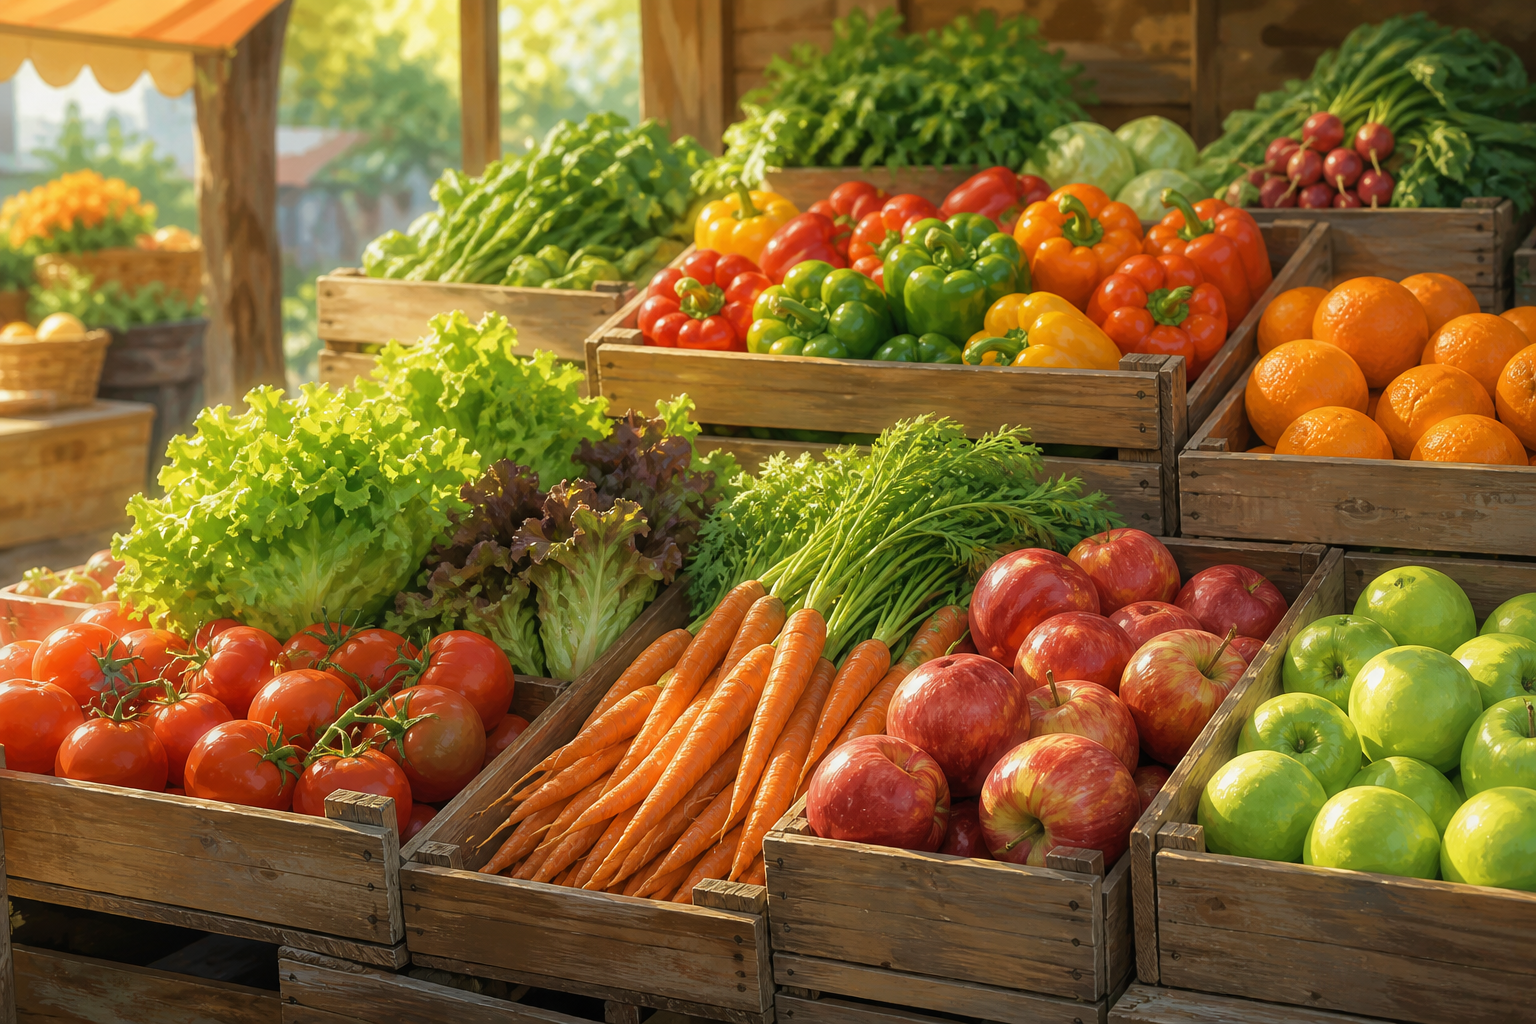
\includegraphics[width=0.62\linewidth]{images/book1/ai/g3-diet-market.png}

{\small A família do frescor na feira: o canto do prato mais
esquecido de todos, aqui sem nenhum risco de passar batido.}
\end{omfigure}

\begin{omfigure}
\begin{tikzpicture}
  % plate
  \draw[thick] (0,0) circle (2.8);
  % half: vegetables/fruit
  \draw[thick, fill=omMeth!14] (0,0) -- (0,2.8)
    arc[start angle=90, end angle=270, radius=2.8] -- cycle;
  % quarter: starchy
  \draw[thick, fill=omProp!14] (0,0) -- (0,-2.8)
    arc[start angle=270, end angle=340, radius=2.8] -- cycle;
  % quarter: builders
  \draw[thick, fill=omThm!12] (0,0) -- ({2.8*cos(340)},{2.8*sin(340)})
    arc[start angle=-20, end angle=90, radius=2.8] -- cycle;
  \node[font=\small, align=center] at (-1.4,0.2)
    {frutas e\\ verduras\\ (metade do prato)};
  \node[font=\small, align=center] at (1.0,-1.45)
    {pão,\\ massa, arroz};
  \node[font=\small, align=center] at (1.3,1.0)
    {carne, peixe,\\ ovo ou laticínio};
  % water glass
  \draw[thick] (4.0,-0.5) -- (4.1,1.0) -- (5.0,1.0) -- (5.1,-0.5)
    -- cycle;
  \fill[omDef!25] (4.04,-0.44) -- (4.12,0.75) -- (4.98,0.75)
    -- (5.06,-0.44) -- cycle;
  \node[font=\small, align=center] at (4.55,-1.0) {água};
\end{tikzpicture}

{\small Um prato bem equilibrado: metade de frescor, um quarto de
\omterm{prop:g3:balanced-diet:jobs}{energia} que dura, um quarto de construtores --- e água no copo.}
\end{omfigure}

\begin{example}[Equilibrando um almoço]\label{ex:g3:balanced-diet:lunch}
Massa com molho de tomate, um pedaço de peixe, vagem, um iogurte,
uma maçã, água: todas as famílias presentes, guloseimas ausentes ---
um almoço equilibrado. Batata frita, refrigerante e uma barra de
chocolate alimentam exatamente duas famílias (gorduras e açúcar) e
pulam justamente as que a obra estava esperando.
\end{example}

\begin{remark}[Não há alimentos proibidos, só esquecidos]\label{rem:g3:balanced-diet:balance}
O equilíbrio é medido em dias, e não em mordidas. Uma fatia de bolo
de aniversário não quebra regra nenhuma --- o problema nunca é uma
guloseima, é guloseima \emph{no lugar} das famílias, dia após dia. A
pergunta prática em cada refeição não é ``esse alimento é ruim?'',
mas ``de que família eu me esqueci hoje?''.
\end{remark}

\section{Ajustar o alimento ao dia}

\begin{proposition}[As necessidades mudam com o dia e com a pessoa]\label{prop:g3:balanced-diet:needs}
Quanta \omterm{prop:g3:balanced-diet:jobs}{energia} um corpo precisa depende de quem ele é e do que ele
faz: uma criança em crescimento precisa proporcionalmente de mais
material de construção do que um adulto; um dia de esporte ou de
frio de inverno queima mais \omterm{prop:g3:balanced-diet:jobs}{energia} do que uma tarde de leitura. A
fome cresce junto com o gasto do corpo.
\end{proposition}
\admitted

\begin{example}[Por que o café da manhã importa]\label{ex:g3:balanced-diet:breakfast}
Pela manhã, o corpo passou a noite inteira funcionando --- coração,
respiração, calor --- sem entrega nenhuma. O café da manhã reabastece
o corpo para as aulas e as correrias da manhã. Pule esse café e, no
meio da manhã, a obra fica no vermelho: barriga roncando, atenção
fugindo, nenhuma força na hora de brincar.
\end{example}

\begin{method}[Conferir o equilíbrio de um dia]\label{met:g3:balanced-diet:check}
No fim do dia, passe pela lista:
\begin{enumerate}
  \item teve fruta ou verdura em todas as refeições? (meta: umas
        cinco porções no dia)
  \item teve alimento que enche em cada refeição, para a \omterm{prop:g3:balanced-diet:jobs}{energia}
        que dura?
  \item os construtores apareceram --- laticínio algumas vezes, e
        carne, peixe ou \omterm{def:g2:animals-grow-up:born}{ovo} uma ou duas vezes?
  \item a água foi a bebida do dia?
  \item as guloseimas: uma quantidade pequena, e não a parte
        principal?
\end{enumerate}
Seja qual for a família que faltou, convide ela amanhã.
\end{method}

\section{Exercícios}

\begin{exercise}[$\star$]\label{exo:g3:balanced-diet:1}
Quais são os dois trabalhos do alimento? Dê uma \omterm{def:g3:balanced-diet:families}{família de alimentos}
que serve principalmente a cada trabalho.
\end{exercise}

\begin{exercise}[$\star$]\label{exo:g3:balanced-diet:2}
Diga as \omterm{def:g3:balanced-diet:families}{famílias de alimentos} e a única bebida de que o corpo
precisa.
\end{exercise}

\begin{exercise}[$\star$]\label{exo:g3:balanced-diet:3}
Separe estas compras em famílias: arroz, iogurte, cenoura, \omterm{def:g2:animals-grow-up:born}{ovo},
manteiga, maçã, pão.
\end{exercise}

\begin{exercise}[$\star$]\label{exo:g3:balanced-diet:4}
Por que o corpo gasta \omterm{prop:g3:balanced-diet:jobs}{energia} até durante o \omterm{prop:g1:healthy-habits:needs}{sono}? Diga duas despesas
da noite.
\end{exercise}

\begin{exercise}[$\star$]\label{exo:g3:balanced-diet:5}
Confira o almoço ``massa, peixe, vagem, iogurte, maçã, água'' com o
prato equilibrado da figura: de que parte do prato é cada item?
\end{exercise}

\begin{exercise}[$\star$]\label{exo:g3:balanced-diet:6}
Por que o café da manhã é especialmente importante? O que acontece
no meio da manhã sem ele?
\end{exercise}

\begin{exercise}[$\star$]\label{exo:g3:balanced-diet:7}
Quem precisa proporcionalmente de mais material de construção: uma
criança ou um adulto? Por quê?
\end{exercise}

\begin{exercise}[$\star$]\label{exo:g3:balanced-diet:8}
Faça a experiência: rode o \cref{met:g3:balanced-diet:check} no seu
próprio dia, com sinceridade. De que família você se esqueceu --- e
qual apareceu mais do que devia?
\end{exercise}

\begin{exercise}[$\star\star$]\label{exo:g3:balanced-diet:9}
``Doce é proibido!'' É isso que este capítulo diz? Dê a regra mais
precisa da \cref{rem:g3:balanced-diet:balance}.
\end{exercise}

\begin{exercise}[$\star\star$]\label{exo:g3:balanced-diet:10}
Numas férias na neve, todo mundo fica com mais fome do que em casa.
Explique com a \cref{prop:g3:balanced-diet:needs} --- diga as duas
despesas a mais que um dia frio e esportivo acrescenta.
\end{exercise}
